%%%%%%%%%%%%%%%%%%%%%%%%%%%%%%%%%%%%%%%%%%%
%%%%%%%%%%%%%%%%%%%%%%%%%%%%%%%%%%%%%%%%%%%
%%%%%%%%%%%%%%% CHAPTER 06 %%%%%%%%%%%%%%%%


\section{Modelagem: sistemas mecânicos de rotação}

\frame{
\frametitle{Variáveis}
\begin{block}{Símbolos utilizados}
\begin{itemize}
    \item Os símbolos para as variáveis básicas utilizadas para descrever o comportamento de um sistema mecânico rotacional são:
    \begin{itemize}
        \item $\theta$, \textbf{deslocamento angular} em radianos (rad)
        \item $\omega$, \textbf{velocidade angular} em radianos por segundo (rad/s)
        \item $\alpha$, \textbf{aceleração angular} em radianos por segundo ao quadrado (rad/s$^2$)
        \item $\tau$, \textbf{torque} em newtons vezes metro (N$\cdot$m)
    \end{itemize}
\end{itemize}
\end{block}
}

\frame{
\frametitle{Variáveis}
\begin{block}{Deslocamento}
\begin{itemize}
    \item Deslocamentos angulares são medidos em relação a um ângulo de \textbf{referência}, que geralmente é a \textbf{orientação de equilíbrio} do corpo ou do ponto.
    \begin{itemize}
        \item Por convenção adota-se as mesmas direções para o deslocamento, velocidade e aceleração angular. Deste modo:
    \end{itemize}
    \vspace{0.2cm}
        $$\omega = \dot{\theta}$$
        $$\alpha = \dot{\omega} = \ddot{\theta}$$
\end{itemize}
\end{block}
\vspace{0.2cm}
\centerline{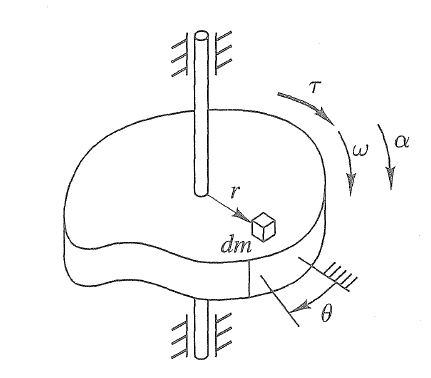
\includegraphics[width=0.3\linewidth]{Figuras/Ch06/fig1.PNG}}
}

\frame{
\frametitle{Leis dos elementos}
\begin{block}{Momento de inércia}
\begin{itemize}
    \item Em mecânica, o momento de inércia ($J$) expressa o \textbf{grau de dificuldade em se alterar o estado de movimento de um corpo em rotação}.
    \item Por definição, o momento de inércia de uma partícula de massa $m$ que gira em torno de um eixo, a uma distância $r$ dele, é:
    $$J = mr^2$$
    \item Se um corpo é constituído de $n$ massas pontuais (partículas), seu momento de inércia total é igual à soma dos momentos de inércia de cada massa:
    $$J = \sum_{i=1}^{n} m_i r_i^2$$
\end{itemize}
\end{block}
}

\frame{
\frametitle{Leis dos elementos}
\begin{block}{Momento de inércia}
\begin{itemize}
    \item Para um corpo rígido, podemos transformar o somatório em uma integral, integrando para todo o corpo o produto da massa $m$ em cada ponto pelo quadrado da distância $r$ até o eixo de rotação:
    $$J = \int_{}^{} r^2 dm$$
    \item Neste curso iremos considerar apenas sistemas não relativístico e momentos de inércia constantes, então:
    $$\tau = J \dot{\omega}$$
\end{itemize}
\end{block}
}

\frame{
\frametitle{Leis dos elementos}
\begin{block}{Atrito}
\begin{itemize}
    \item Um elemento de atrito rotacional é aquele onde existe uma relação algébrica entre o \textbf{torque} e a \textbf{velocidade angular} relativa entre dois corpos.
    \item O momento de inércia deste elemento é negligenciável ou representado separadamente, por isso, podemos concluir que os torques aplicados nas duas extremidades do elemento devem ser \textbf{iguais em magnitude e com direções opostas}.
    $$\tau = B\Delta \omega$$
onde $B$ é o coeficiente de atrito (N$\cdot$s$\cdot$m) e $\Delta \omega = \omega_2 - \omega_1$
$$\tau = B (\omega_2 - \omega_1)= B (\dot{\theta}_2-\dot{\theta}_1)$$
\end{itemize}
\end{block}
\vspace{-0.05cm}
\centerline{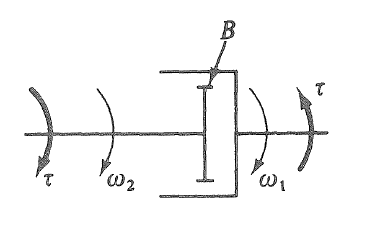
\includegraphics[width=0.23\linewidth]{Figuras/Ch06/fig2.PNG}}
}

\frame{
\frametitle{Leis dos elementos}
\begin{block}{Rigidez}
\begin{itemize}
    \item A rigidez rotacional está basicamente associada a uma \textbf{mola de torção}. Este elemento pode ser descrito através de uma relação algébrica entre $\tau$ e $\theta$
    \item O momento de inércia deste elemento é negligenciável ou representado separadamente, por isso, podemos concluir que os torques aplicados nas duas extremidades do elemento devem ser \textbf{iguais em magnitude e com direções opostas}.
$$\tau = K\Delta \theta$$
onde $K$ é a constante de rigidez da mola (N$\cdot$m) e $\Delta \theta = \theta_2 - \theta_1$
$$\tau = K (\theta_2 - \theta_1)$$
\end{itemize}
\end{block}
\centerline{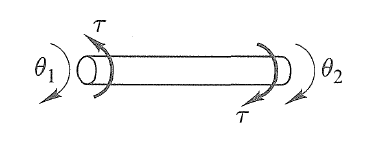
\includegraphics[width=0.35\linewidth]{Figuras/Ch06/fig3.PNG}}
}

\frame{
\frametitle{Leis dos elementos}
\begin{block}{Alavanca ideal}
\begin{itemize}
    \item Uma \textbf{alavanca ideal} é aquela considerada sem massa, sem atrito, sem momento de inércia e sem energia armazenada.
    \item Em nosso curso o \textbf{ponto de pivô} será sempre \textbf{fixo}.
$$x_1 = d_1 \cdot sen\theta \qquad x_2 = d_2 \cdot sen \theta$$
Para pequenos deslocamentos, tem-se:
$$x_1 \approx d_1 \cdot \theta \qquad x_2 \approx d_2 \cdot \theta$$
\end{itemize}
\end{block}
\centerline{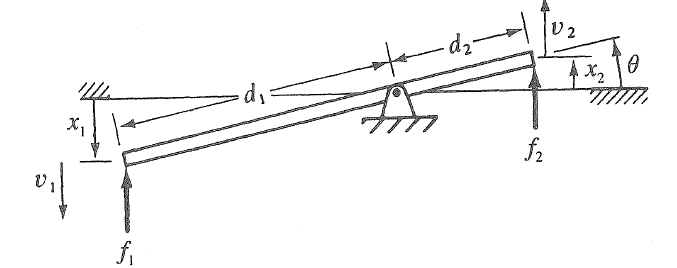
\includegraphics[width=0.65\linewidth]{Figuras/Ch06/fig4.PNG}}
}

\frame{
\frametitle{Leis dos elementos}
\begin{block}{Alavanca ideal}
\begin{itemize}
    \item Assim:
$$\theta = \dfrac{x_1}{d_1} = \dfrac{x_2}{d_2} \implies x_2 = \dfrac{d_2}{d_1}x_1$$
    \item Desconsiderando-se a massa da alavanca, tem-se a soma dos momentos em torno do ponto de pivotamento como:
$$f_2d_2 - f_1d_1 = 0 \implies f_2 = \dfrac{d_1}{d_2}f_1$$
    \item O pivô exerce uma \textbf{força} de valor $f_1 + f_2$ na alavanca, mas isto não é levado em consideração na hora da derivação da fórmula anterior, visto que esta força não exerce nenhum momento no pivô.
\end{itemize}
\end{block}
}

\frame{
\frametitle{Leis dos elementos}
\begin{block}{Engrenagem}
\begin{itemize}
    \item Uma \textbf{engrenagem ideal} é aquela considerada sem atrito, sem momento de inércia, sem energia armazenada e com um perfeito encaixe de seus dentes.
    \item Considerando $r$ como o raio da engrenagem e $n$ como o número de dentes da mesma, temos:
$$\dfrac{r_2}{r_1} = \dfrac{n_2}{n_1} = N$$
onde $N$ é \textbf{razão da engrenagem}. 
\end{itemize}
\end{block}
\centerline{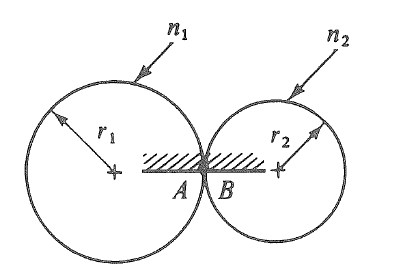
\includegraphics[width=0.35\linewidth]{Figuras/Ch06/fig5.PNG}}
}

\frame{
\frametitle{Leis dos elementos}
\begin{block}{Engrenagem}
\begin{itemize}
    \item Após a rotação, o tamanho do arco $PA$ deve ser igual ao tamanho do arco $PB$:
$$\dfrac{\theta_1}{\theta_2} = \dfrac{r_2}{r_1} = N$$
    \item Diferenciando no tempo a equação acima, podemos perceber que as velocidades angulares também estão relacionadas com a razão da engrenagem:
$$\dfrac{\omega_1}{\omega_2} = \dfrac{r_2}{r_1} = N$$
\end{itemize}
\end{block}
\centerline{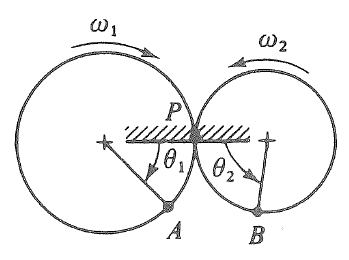
\includegraphics[width=0.35\linewidth]{Figuras/Ch06/fig6.PNG}}
}

\frame{
\frametitle{Leis dos elementos}
\begin{block}{Engrenagem}
\begin{itemize}
    \item Os torques externos aplicados são $\tau_1$ e $\tau_2$.
    \item A força exercida por cada engrenagem no ponto de contato é $f_c$. De acordo com a lei da ação e reação, as setas devem estar em \textbf{direções opostas} em cada engrenagem.
    \item Desconsiderando-se a inércia da engrenagem, tem-se que a soma dos torques em cada engrenagem deve ser igual a 0. Eliminando $f_c$ obtemos:
$$\dfrac{\tau_2}{\tau_1} = -\dfrac{r_2}{r_1} = -N$$
\end{itemize}
\end{block}
\centerline{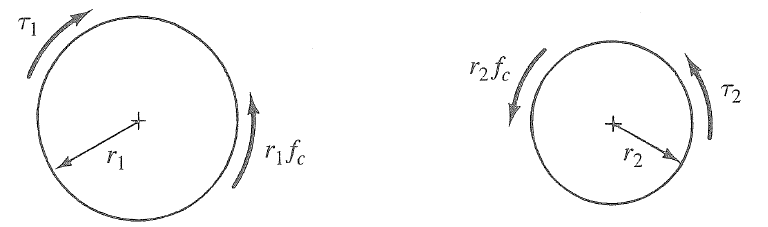
\includegraphics[width=0.7\linewidth]{Figuras/Ch06/fig7.PNG}}
}

\frame{
\frametitle{Interconectando as leis}
\begin{block}{Lei de D'Alembert}
\begin{itemize}
    \item A lei de D'Alembert é apenas uma reorganização da segunda lei de Newton. Ela diz que a soma dos momentos em um ponto particular P terá uma resultante nula.
    \item Considerando o nosso caso em estudo, tal lei nos diz que a soma algébrica de todas os torques aplicados externamente em um corpo e do torque de inércia (que resiste ao movimento rotacional do corpo) em uma direção particular é zero.
\end{itemize}
$$\sum_{i}^{} (\tau_{ext})_i = J \dot{\omega} \implies \sum_{i}^{} (\tau_{ext})_i - J \dot{\omega} = 0$$
$$\boxed{\sum_{i}^{} \tau_i = 0}$$
\end{block}
}

\frame{
\frametitle{Exemplo $\#01$ - sistema rotacional simples}
\centerline{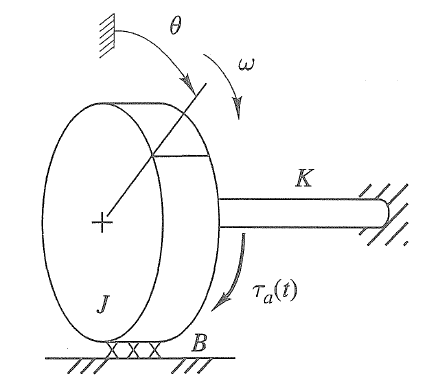
\includegraphics[width=0.25\linewidth]{Figuras/Ch06/fig8.PNG}}
\begin{block}{Problema}
\begin{itemize}
    \item Análise feita no disco com \textbf{momento de inércia} $\bm{J}$.
    \item Movimento rotacional no sentido horário.
    \item Os torques são:
    \begin{itemize}
        \item $\bm{\tau_K}$: torque exercido pela mola torcional. Este deve estar no sentido \textbf{anti-horário}, já que $\theta$ movimenta-se no sentido horário.
        \item $\bm{\tau_B}$: torque exercido pelo amortecedor. Também deve estar no sentido \textbf{anti-horário}.
        \item $\bm{\tau_I}$: torque de inércia. Este torque também se encontra no sentido \textbf{anti-horário}, se opondo ao movimento do corpo.
        \item $\bm{\tau_a(t)}$: torque aplicado ao sistema, no \textbf{sentido horário}.
    \end{itemize}
\end{itemize}
\end{block}
}

\frame{
\frametitle{Exemplo $\#01$ - sistema rotacional simples}
\centerline{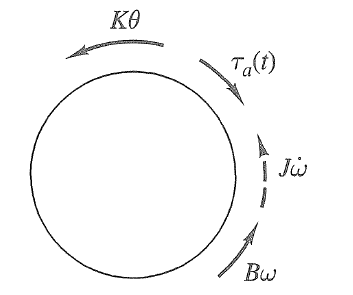
\includegraphics[width=0.3\linewidth]{Figuras/Ch06/fig9.PNG}}
\begin{block}{Diagrama de corpo livre}
\begin{itemize}
    \item Aplicando a lei de D'Alembert, \textbf{respeitando as direções assumidas}, e considerando que os torques agindo no sentido horário são positivos, obtemos:
$$\tau_a(t) - (J\dot{\omega} + B\omega + K\theta) = 0$$
Substituindo $\omega$ por $\dot{\theta}$ e $\dot{\omega}$ por $\ddot{\theta}$, e rearranjando os termos, temos:
$$J\ddot{\theta} + B\dot{\theta} + K\theta = \tau_a(t)$$
\end{itemize}
\end{block}
}

\frame{
\frametitle{Exemplo $\#02$ - sistema rotacional com dois discos interconectados}
\centerline{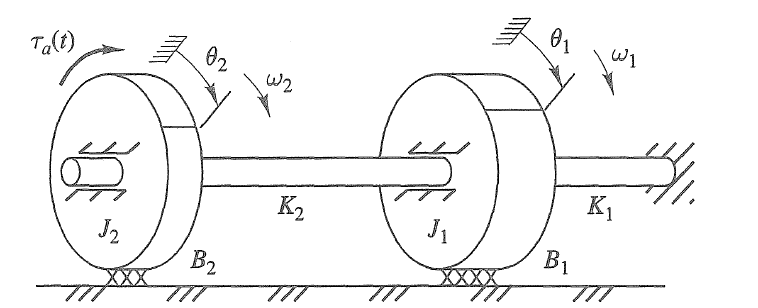
\includegraphics[width=0.4\linewidth]{Figuras/Ch06/fig10.PNG}}
\begin{block}{Problema}
\begin{itemize}
    \item A análise deve ser feita \textbf{separadamente} nos dois discos com \textbf{momento de inércia} $\bm{J_1}$ e $\bm{J_2}$ (podem se mover com velocidades angulares desconhecidas diferentes).
    \item Para o primeiro disco com momento de inércia $\bm{J_1}$ \textbf{(considere} $\bm{\theta_2 > \theta_1)}$:
    \begin{itemize}
        \item O torque exercido pela mola torcional $\bm{K_1\theta_1}$ atua apenas no disco 1, no sentido anti-horário.
        \item O torque exercido pelo amortecimento $\bm{B_1\omega_1}$ atua apenas no disco 1, no sentido anti-horário.
        \item Do mesmo modo acontece com o torque inercial $\bm{J_1\dot{\omega}_1}$.
        \item A parcela $\bm{K_2(\theta_2-\theta_1)}$, considerando a rigidez torcional entre os dois discos e lembrando que $\theta_2 > \theta_1$ (por hipótese), resulta em um torque no sentido horário.
    \end{itemize}
\end{itemize}
\end{block}
}

\frame{
\frametitle{Exemplo $\#02$ - sistema rotacional com dois discos interconectados}
\centerline{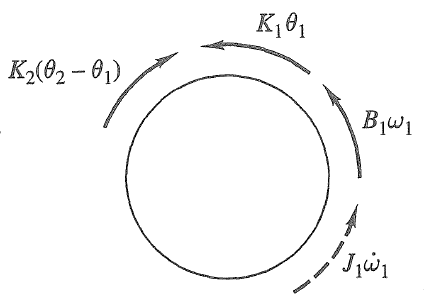
\includegraphics[width=0.4\linewidth]{Figuras/Ch06/fig12.PNG}}
\begin{block}{Diagrama de corpo livre}
\begin{itemize}
    \item Aplicando a lei de D'Alembert, \textbf{respeitando as direções assumidas}, e considerando que os torques agindo no sentido horário são positivos, obtemos:
$$-J_1\dot{\omega}_1 - B_1\omega_1 - K_1\theta_1 + K_2(\theta_2 - \theta_1) = 0$$
Rearranjando os termos, temos:
$$J_1\ddot{\theta}_1 + B_1\dot{\theta}_1 + (K_1 + K_2)\theta_1 - K_2\theta_2 = 0$$
\end{itemize}
\end{block}
}

\frame{
\frametitle{Exemplo $\#02$ - sistema rotacional com dois discos interconectados}
\centerline{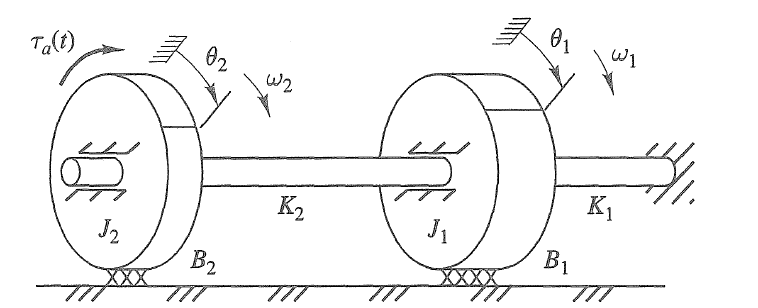
\includegraphics[width=0.4\linewidth]{Figuras/Ch06/fig10.PNG}}
\begin{block}{Problema}
\begin{itemize}
    \item A análise deve ser feita \textbf{separadamente} nos dois discos com \textbf{momento de inércia} $\bm{J_1}$ e $\bm{J_2}$ (podem se mover com velocidades angulares desconhecidas diferentes).
    \item Para o segundo disco com momento de inércia $\bm{J_2}$ \textbf{(obrigatoriamente deve-se continuar considerando} $\bm{\theta_2 > \theta_1)}$:
    \begin{itemize}
        \item O torque exercido pelo amortecimento $\bm{B_2\omega_2}$ atua apenas no disco 2, no sentido anti-horário.
        \item Do mesmo modo acontece com o torque inercial $\bm{J_2\dot{\omega}_2}$.
        \item A parcela $\bm{K_2(\theta_2-\theta_1)}$, considerando a rigidez torcional entre os dois discos e lembrando que $\theta_2 > \theta_1$ (por hipótese), resulta em um torque no sentido anti-horário (lei da ação e reação, visto que no disco 1 este torque está no sentido horário).
        \item O torque aplicado $\tau_a(t)$ está no sentido horário.
    \end{itemize}
\end{itemize}
\end{block}
}

\frame{
\frametitle{Exemplo $\#02$ - sistema rotacional com dois discos interconectados}
\centerline{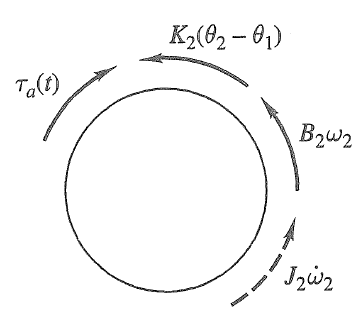
\includegraphics[width=0.3\linewidth]{Figuras/Ch06/fig11.PNG}}
\begin{block}{Diagrama de corpo livre}
\begin{itemize}
    \item Aplicando a lei de D'Alembert, \textbf{respeitando as direções assumidas}, e considerando que os torques agindo no sentido horário são positivos, obtemos:
$$-J_2\dot{\omega}_2 - B_2\omega_2 - K_2(\theta_2 - \theta_1) + \tau_a(t) = 0$$
Rearranjando os termos, temos:
$$-K_2\theta_1 + J_2\ddot{\theta}_2 + B_2\dot{\theta}_2 + K_2\theta_2= \tau_a(t)$$
\end{itemize}
\end{block}
}

\frame{
\frametitle{Exemplo $\#02$ - sistema rotacional com dois discos interconectados}
\begin{block}{EDOs}
\begin{equation*}
\begin{cases}
J_1\ddot{\theta}_1 + B_1\dot{\theta}_1 + (K_1 + K_2)\theta_1 - K_2\theta_2 = 0 \\
-K_2\theta_1 + J_2\ddot{\theta}_2 + B_2\dot{\theta}_2 + K_2\theta_2= \tau_a(t)
\end{cases}
\end{equation*}
\begin{itemize}
    \item Caso seja pedido uma equação que relaciona a saída desejada ($\theta_2$, por exemplo) com a entrada aplicada $\tau_a(t)$, deve-se isolar $\theta_1$ na segunda equação, e substituir na primeira equação, realizando as devidas derivadas e cálculos necessários (\textit{à cargo do leitor, com resposta na página 107 do livro texto}).
\end{itemize}
\end{block}
}

\frame{
\frametitle{Exemplo $\#03$ - sistema rotacional com elementos em série}
\centerline{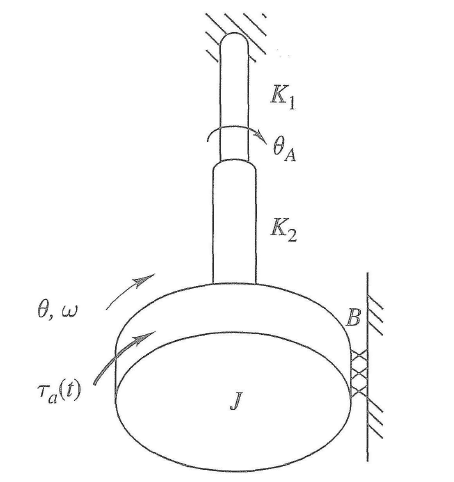
\includegraphics[width=0.4\linewidth]{Figuras/Ch06/fig13.PNG}}
\begin{block}{Problema}
\begin{itemize}
    \item A ideia deste exemplo é encontrar um \textbf{elemento de rigidez único} que substitua as duas partes mostradas na imagem acima.
    \item $\tau_r$ é o torque de \textbf{reação} aplicado pelo suporte sobre o eixo, contrário ao movimento de $\theta_A$
\end{itemize}
\end{block}
}

\frame{
\frametitle{Exemplo $\#03$ - sistema rotacional com elementos em série}
\centerline{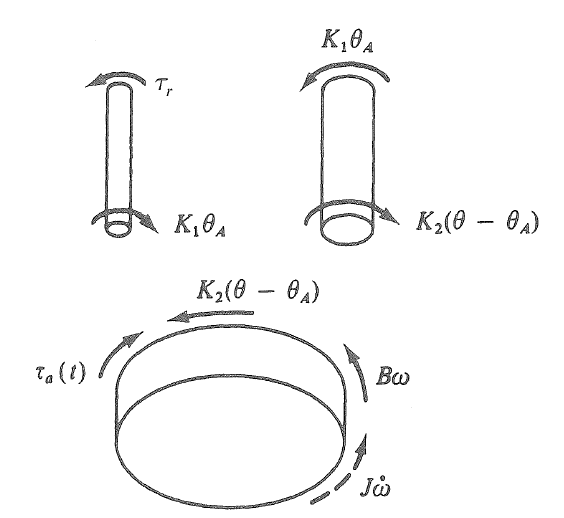
\includegraphics[width=0.45\linewidth]{Figuras/Ch06/fig14.PNG}}
\begin{block}{Diagrama de corpo livre}
\begin{equation*}
\begin{cases}
K_1\theta_A - \tau_r = 0 \\
K_2(\theta - \theta_A) - K_1\theta_A = 0 \\
-J\dot{\omega} - B\omega - K_2(\theta - \theta_A) + \tau_a(t) = 0
\end{cases}
\end{equation*}
\end{block}
}

\frame{
\frametitle{Exemplo $\#03$ - sistema rotacional com elementos em série}
\begin{block}{Conclusão}
Da segunda equação obtemos $\theta_A = \Big(\dfrac{K_2}{K_1 + K_2}\Big)\theta$ \\
\vspace{0.2cm}
Substituindo essa relação na terceira equação, e rearrumando os termos, temos:
$$J\dot{\omega} + B\omega + K_{eq} \theta = \tau_a(t) $$
onde 
$$\boxed{K_{eq} = \dfrac{K_1K_2}{K_1+K_2}}$$
\end{block}
}

\frame{
\frametitle{Exemplo $\#04$ - sistema rotacional com alavanca ideal}
\centerline{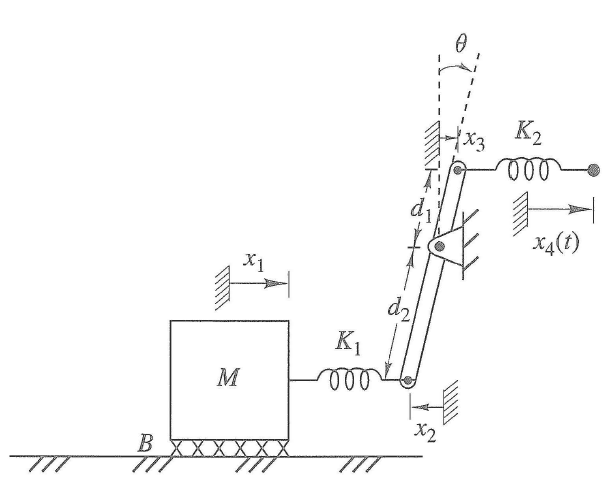
\includegraphics[width=0.55\linewidth]{Figuras/Ch06/fig15.PNG}}
\begin{block}{Problema}
\begin{itemize}
    \item Neste exemplo uma atenção especial deve ser dada para os sinais referentes a deformação da mola, devido ao modo em que os deslocamentos foram definidos.
\end{itemize}
\end{block}
}

\frame{
\frametitle{Exemplo $\#04$ - sistema rotacional com alavanca ideal}
\centerline{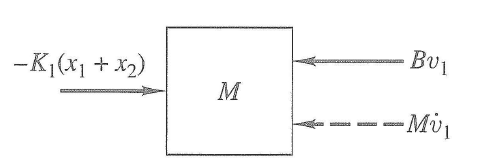
\includegraphics[width=0.45\linewidth]{Figuras/Ch06/fig16.PNG}}
\begin{block}{Diagrama de corpo livre}
\begin{itemize}
    \item Aplicando a lei de D'Alembert, \textbf{respeitando as direções assumidas}, e considerando que as forças agindo para direita são positivas, obtemos:
$$-K_1(x_1 + x_2) - Bv_1 - M\dot{v}_1 = 0$$
Rearranjando os termos, temos:
$$M\dot{v}_1 + Bv_1 + K_1(x_1 + x_2) = 0$$
\end{itemize}
\end{block}
}

\frame{
\frametitle{Exemplo $\#04$ - sistema rotacional com alavanca ideal}
\centerline{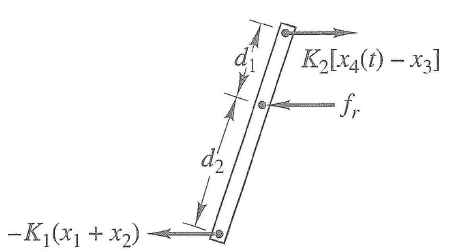
\includegraphics[width=0.35\linewidth]{Figuras/Ch06/fig17.PNG}}
\begin{block}{Diagrama de corpo livre}
\begin{itemize}
    \item Considerando um ângulo de rotação $\theta$ pequeno, temos:
    $$x_3 = \big(\dfrac{d_1}{d_2}\big)x_2$$
    \item A soma dos momentos em torno do ponto de pivotamento é:
    $$K_2[x_4(t) - x_3]d_1 - K_1(x_1+x_2)d_2 = 0$$
    \item A soma das forças na alavanca é dada por:
    $$f_r = K_2[x_4(t) - x_3] + K_1(x_1+x_2)$$
\end{itemize}
\end{block}
}

\frame{
\frametitle{Exemplo $\#05$ - sistema rotacional com engrenagem}
\centerline{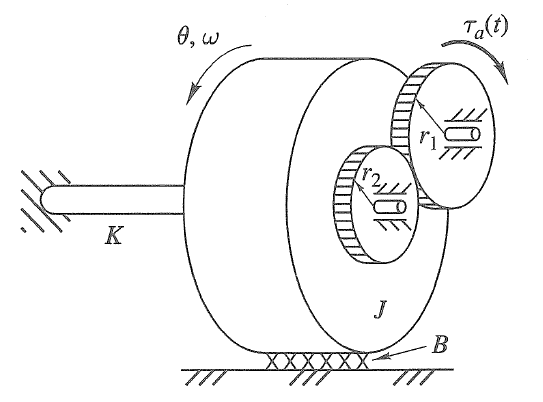
\includegraphics[width=0.55\linewidth]{Figuras/Ch06/fig18.PNG}}
\begin{block}{Problema}
\begin{itemize}
    \item Quando uma engrenagem está conectada a um sistema, ela pode mudar a \textbf{magnitude do torque} aplicado ao corpo em rotação, além de \textbf{reverter a direção do disco}.
\end{itemize}
\end{block}
}

\frame{
\frametitle{Exemplo $\#05$ - sistema rotacional com engrenagem}
\centerline{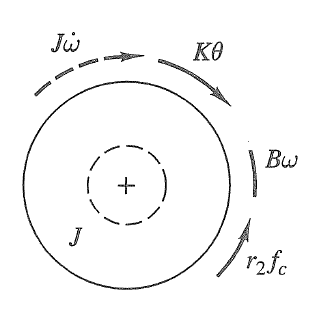
\includegraphics[width=0.3\linewidth]{Figuras/Ch06/fig19.PNG}}
\begin{block}{Diagrama de corpo livre}
\begin{itemize}
    \item Aplicando a lei de D'Alembert, \textbf{respeitando as direções assumidas}, e considerando que os torques agindo no sentido horário são positivos, obtemos:
$$J\dot{\omega} + B\omega + K\theta - r_2f_c = 0$$
Rearranjando os termos, temos:
$$J\ddot{\theta} + B\dot{\theta} + K\theta - r_2f_c = 0$$
\end{itemize}
\end{block}
}

\frame{
\frametitle{Exemplo $\#05$ - sistema rotacional com engrenagem}
\centerline{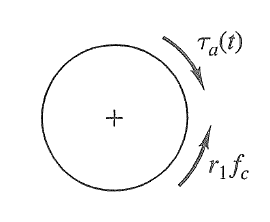
\includegraphics[width=0.3\linewidth]{Figuras/Ch06/fig20.PNG}}
\begin{block}{Diagrama de corpo livre}
\begin{itemize}
    \item Aplicando a lei de D'Alembert, \textbf{respeitando as direções assumidas}, e considerando que os torques agindo no sentido horário são positivos, obtemos:
$$\tau_a(t) - r_1f_c = 0$$
Rearranjando os termos, temos:
$$r_1f_c = \tau_a(t)$$
\end{itemize}
\end{block}
}

\frame{
\frametitle{Exemplo $\#05$ - sistema rotacional com engrenagem}
\begin{block}{Conclusão}
\begin{itemize}
    \item Isolando $f_c$ na segunda equação, temos:
$$f_c = \dfrac{\tau_a(t)}{r_1}$$
Substituindo esta última relação na primeira equação, obtemos:
$$J\ddot{\theta} + B\dot{\theta} + K\theta - r_2 \Big(\dfrac{\tau_a(t)}{r_1}\Big)= 0$$
$$J\ddot{\theta} + B\dot{\theta} + K\theta = r_2 \Big(\dfrac{\tau_a(t)}{r_1}\Big)$$
$$J\ddot{\theta} + B\dot{\theta} + K\theta = N\tau_a(t)$$
    \item Comparando esta equação com a do exemplo 1 ($J\ddot{\theta} + B\dot{\theta} + K\theta = \tau_a(t)$) vemos que o único efeito esperado com a adição da engrenagem é multiplicar o torque aplicado $\tau_a(t)$ pela razão de engrenagem $N$, além de mudar a direção de rotação do disco.
\end{itemize}
\end{block}
}

\frame{
\frametitle{Exercícios}
\begin{block}{}
01. Para o sistema mostrado abaixo (à esquerda), desenhe o diagrama de corpo livre e modele-o.

\vspace{0.5cm}

02. Repita para o sistema mostrado à direita.
\end{block}
\centerline{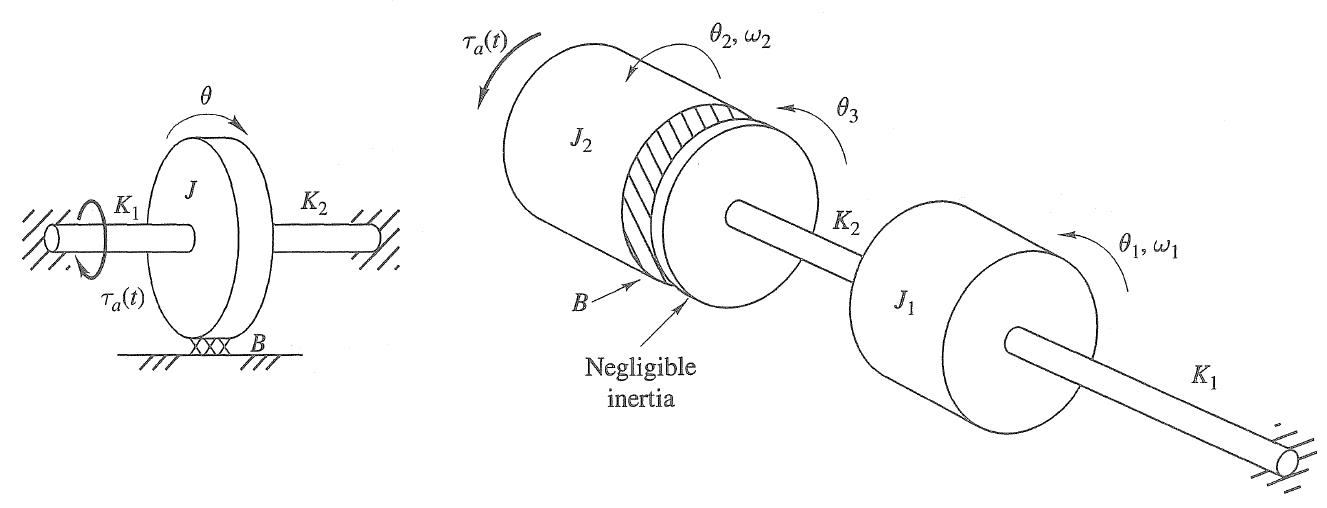
\includegraphics[width=1.1\linewidth]{Figuras/Ch06/fig21.PNG}}
}

\frame{
\frametitle{Referências e exercícios complementares}
\begin{itemize}
\item CLOSE, Charles M.; FREDERICK, Dean K.; NEWELL, Jonathan C. Modeling and Analysis of Dynamic Systems, 3 ed. John Wiley \& Sons, 2003.
\end{itemize}
\centering{\alert{Página 126 - \textbf{Capítulo 5}}} \\
}